\documentclass[a4paper,12pt,abstracton]{scrartcl}
\usepackage[utf8]{inputenc}
\usepackage{float}
\usepackage{tikz}
\usepackage{amsmath}
\usepackage{amssymb}
\usepackage{pifont}% http://ctan.org/pkg/pifont
\usepackage[font=small,labelfont=bf]{caption}
\usepackage{graphicx}
\usepackage{dirtytalk}
\usepackage{multicol}
\usepackage{booktabs}
\usepackage{colortbl}
\usepackage{appendix}
\usepackage{nomencl}
\usepackage{lmodern}
\usepackage[nottoc]{tocbibind}
\usepackage{xcolor}
%\graphicspath{images/}
\usepackage[margin = 3cm]{geometry}
\usepackage{ragged2e} % good alignment
\usepackage{hyperref}
\usepackage{siunitx} % Provides the \SI{}{} and \si{} command for typesetting SI units
\hypersetup{colorlinks=true,
    linkcolor=blue,
    filecolor=magenta,      
    urlcolor=cyan, 
    citecolor=gray}

%\DeclareGraphicsExtensions{.png,.pdf} % low-res (work in progress)
%\DeclareGraphicsExtensions{.pdf,.png}  % high-res (final draft)
%\setlength\parindent{0pt} % Removes all indentation from paragraphs
%\bibliographystyle{unstr}
\setlength\parindent{0pt}
\setlength{\parskip}{0.3em}
\newcommand{\xmark}{\ding{55}}

\begin{document}
\section{Anomalous Zeeman Effect}

\subsection{Data Collection}

The data regarding the transverse and longitudinal configurations have been collected and reported in \hyperref[table:zat]{Table \ref*{table:zat}} and \hyperref[table:zal]{ \ref*{table:zal}} respectively. The values of $B$ have been derived from those of $I$ in \hyperref[sec:cal]{Calibration Curve}, while $\frac{\langle \delta \rangle}{\langle \Delta \rangle}$ has been calculated as described in \hyperref[sec:ExpIntro]{Experimental Introduction}.

\subsection{Data Analysis \& Visualization}

The datasets concerning the transverse and longitudinal configurations have been fit with the linear model $f(B)=\boldsymbol{p_0}B+\boldsymbol{p_1}$ and plotted in \hyperref[fig:zat]{Figure \ref*{fig:zat}} and \hyperref[fig:zal]{ \ref*{fig:zal}}, together with the respective fit parameters $\boldsymbol{p_0}$ and  $\boldsymbol{p_1}$ .


\begin{table}[H]
\centering
\caption{}
\label{table:zat}
\resizebox{8.2cm}{!}{
  \begin{tabular}{cccccc}
  \toprule
 $I\;[A]$ & $B\;[T]$ & $\frac{\langle \delta \rangle}{\langle \Delta \rangle}$ \\
  \midrule
  \rowcolor{gray!6}  5.75 $\pm$ 0.04 & 0.394 $\pm$ 0.041 & 0.062 $\pm$ 0.002\\
  6.74 $\pm$ 0.02 & 0.460 $\pm$ 0.048 & 0.081 $\pm$ 0.021\\
  \rowcolor{gray!6}  7.275 $\pm$ 0.025 & 0.504 $\pm$ 0.052 & 0.098 $\pm$ 0.019\\
  7.82 $\pm$ 0.02 & 0.537 $\pm$ 0.056 & 0.086 $\pm$ 0.034\\
  \rowcolor{gray!6}  8.795 $\pm$ 0.095 & 0.590 $\pm$ 0.061 & 0.096 $\pm$ 0.030\\
  9.95 $\pm$ 0.04 & 0.642 $\pm$ 0.066 & 0.082 $\pm$ 0.032\\
  \bottomrule
  \end{tabular}}
\end{table}

\begin{figure}[H]
     \centering
     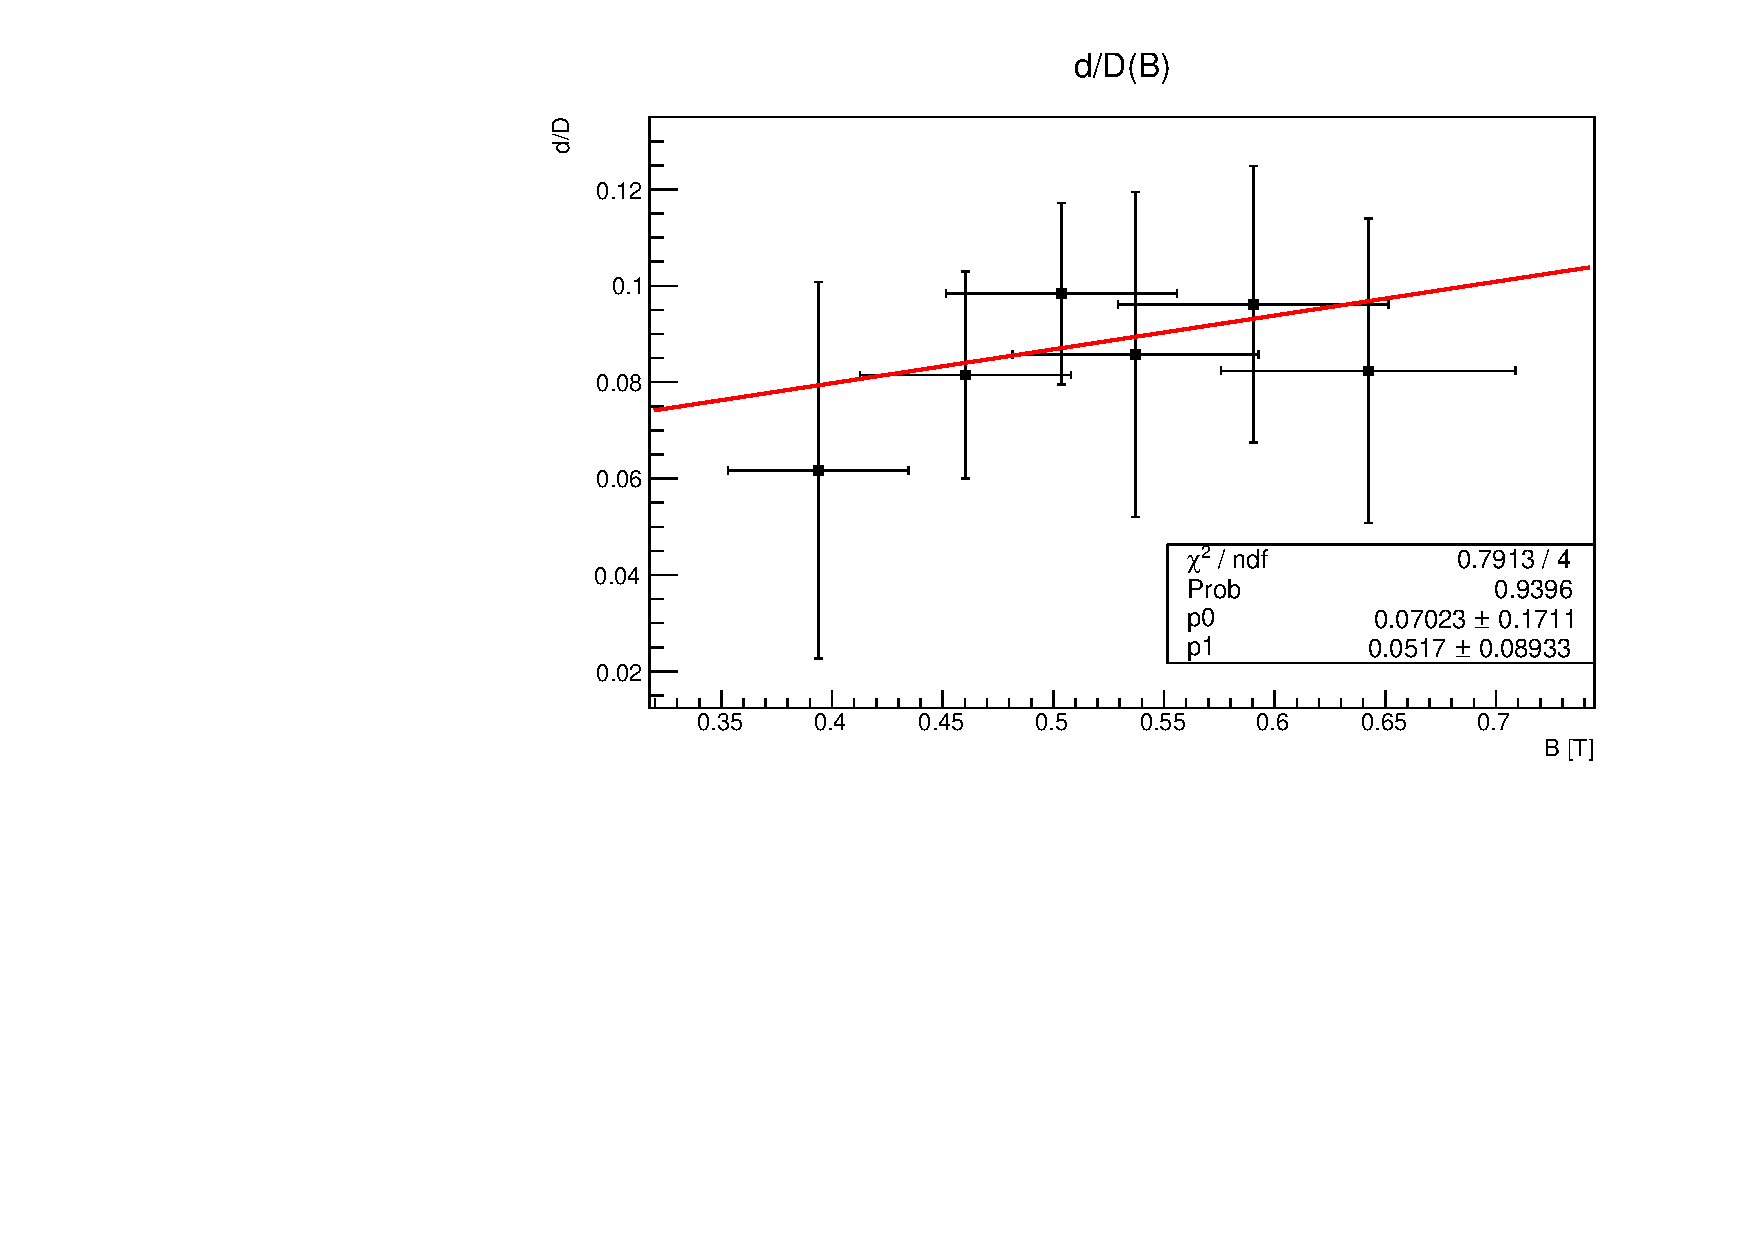
\includegraphics[scale=0.76]{plots/zat.pdf}
    \caption{Transverse}
    \label{fig:zat}
\end{figure}

\begin{table}[H]
\centering
\caption{}
\label{table:zal}
\resizebox{12cm}{!}{
  \begin{tabular}{cccccc}
  \toprule
 $I\;[A]$ & $B\;[T]$ & $\frac{\langle \delta \rangle}{\langle \Delta \rangle}$ \\
  \midrule
  \rowcolor{gray!6}  7.31 $\pm$ 0.02 & 0.506 $\pm$ 0.052 & 0.057 $\pm$ 0.011\\
  7.85 $\pm$ 0.02 & 0.539 $\pm$ 0.056 & 0.069 $\pm$ 0.012\\
  \rowcolor{gray!6}  8.32 $\pm$ 0.02 & 0.565 $\pm$ 0.059 & 0.088 $\pm$ 0.017\\
  8.84 $\pm$ 0.02 & 0.593 $\pm$ 0.061 & 0.128 $\pm$ 0.031\\
  \rowcolor{gray!6}  9.415 $\pm$ 0.025 & 0.620 $\pm$ 0.064 & 0.147 $\pm$ 0.022\\
  9.99 $\pm$ 0.02 & 0.644 $\pm$ 0.067 & 0.130 $\pm$ 0.022\\
  \bottomrule
  \addlinespace
    \addlinespace
  \addlinespace
  \addlinespace
  \addlinespace
  \end{tabular}}
\end{table}
\begin{figure}[H]
   \hspace{-1.7cm} 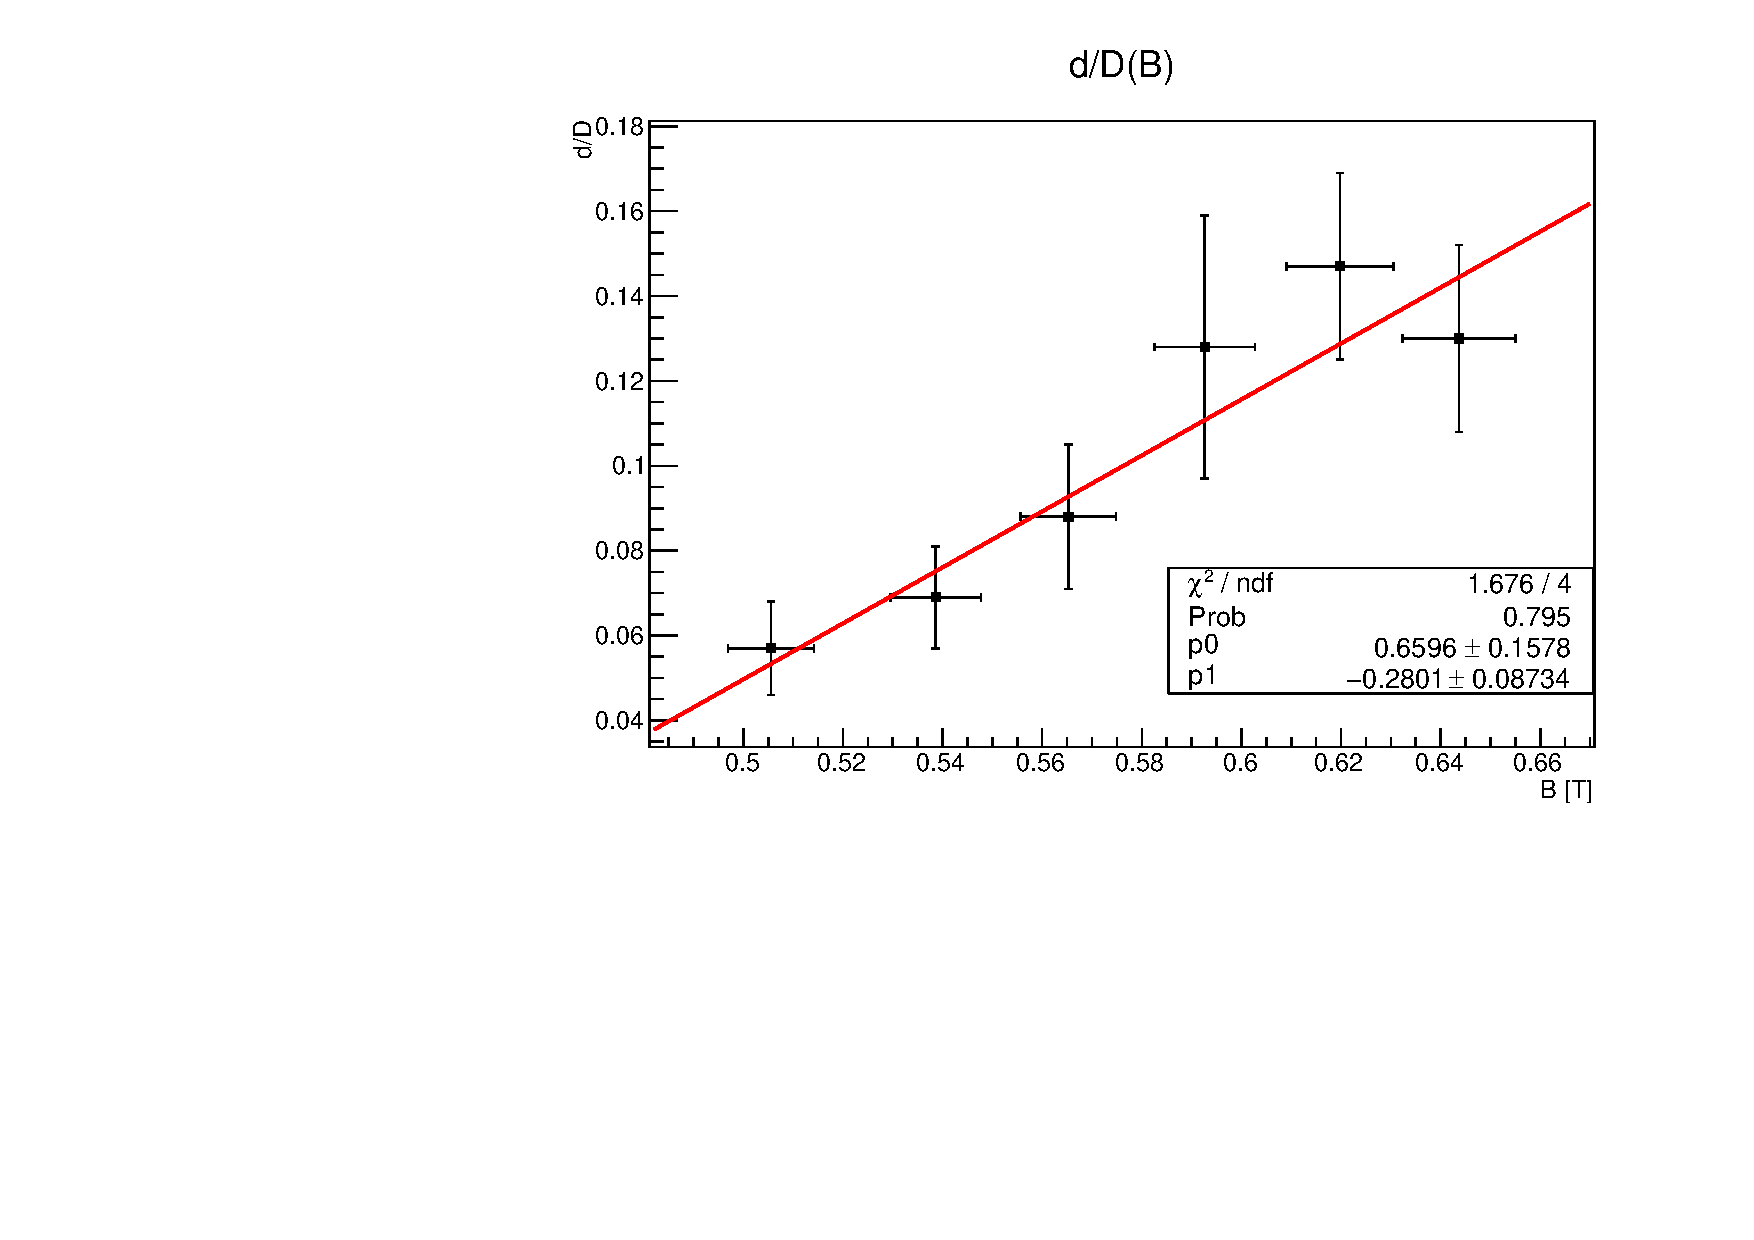
\includegraphics[scale=0.95]{plots/zal.pdf}
    \caption{Longitudinal}
    \label{fig:zal}
\end{figure}

\subsection{Bohr Magneton}
Now it is possible to calculate the Bohr magneton for both configurations $$\mu_A^T= (\boldsymbol{p_0^T}\pm \boldsymbol{\delta p_0^T})\frac{hc}{2g_a\mu_a w} \quad\text{and}\quad \mu_A^L= (\boldsymbol{p_0^L}\pm \boldsymbol{\delta p_0^L})\frac{hc}{2g_a\mu_a w}$$ 
 since we know 
\begin{itemize}
\item $h=6.626070040\times10^{-34} \text{ Js}  \;\,\quad\qquad\qquad\text{ Plack constant}$  
\item $c=299792458 \text{ ms}^{-1}  \quad\qquad\qquad\qquad\qquad\text{speed of light in the vacuum}$
\item $g_a=1/2   \;\;\quad\qquad\qquad\qquad\qquad\qquad\qquad\text{ gyromagnetic factor}$
\item $\mu_a= 1.4560    \;\qquad\qquad\qquad\qquad\qquad\qquad\text{ refractive index}$
\item  $w= 0.003 \text{ m} \;\qquad\qquad\qquad\qquad\qquad\qquad\text{thickness}$
\item $\boldsymbol{p_0^{T}}=0.070 \pm 0.171 \;\text{T}^{-1}
\;\quad\qquad\qquad\qquad\text{ transverse slope}$
\item $\boldsymbol{p_0^{L}}=0.737 \pm 0.433 \;\text{T}^{-1} \;\quad\qquad\qquad\qquad\text{ longitudinal slope .}$\newline
\end{itemize} 

The compatibility between $\mu_A^T$ and $\mu_A^L$ has been tested as displayed in \hyperref[table:Za]{Table \ref*{table:Za}}. 
\begin{table}[H]
\caption{}
\centering
\resizebox{11cm}{!}{
\begin{tabular}{cccc}
\toprule
$\mu_A^T\;[\text{JT}^{-1}]$ & $\mu_A^L\;[\text{JT}^{-1}]$ & $Z$ & Compatibility  \\
\midrule
\rowcolor{gray!6} $3.20 \pm 7.80\times 10^{-24}$ & $33.61 \pm 19.75$ & 1.43 & \checkmark \\
\bottomrule
\end{tabular}}
\label{table:Za}
\end{table}

Since the result has been positive, we have calculated the weighted average $$ \langle \mu_A\rangle=7.30 \pm 7.25\times 10^{-24}\;\text{JT}^{-1}\;.$$

% footnote ZN VS ZA : due to experimental limits (see notes) and expected complications 

Then the compatibility test between $\langle \mu_A \rangle$ and $\langle \mu_N \rangle$ has been computed and displayed in \hyperref[table:Zan]{Table \ref*{table:Zan}}. 
\begin{table}[H]
\caption{}
\centering
\resizebox{11cm}{!}{
\begin{tabular}{cccc}
\toprule
$\langle \mu_A \rangle\;[\text{JT}^{-1}]$ & $\langle \mu_N \rangle\;[\text{JT}^{-1}]$ & $Z$ & Compatibility  \\
\midrule
\rowcolor{gray!6} $7.30 \pm 7.25\times 10^{-24}$ & $9.79 \pm 6.63$ & 0.34 & \checkmark \\
\bottomrule
\end{tabular}}
\label{table:Zan}
\end{table}

Since the result has been positive, we have calculated the global weighted average $$ \langle \mu\rangle=9.77 \pm  0.63\times 10^{-24}\;\text{JT}^{-1}$$ which has been tested against the theoretical value $\boldsymbol{\mu_B}$ as shown in \hyperref[table:Z]{Table \ref*{table:Z}} .

\begin{table}[H]
\caption{}
\centering
\resizebox{11cm}{!}{
\begin{tabular}{cccc}
\toprule
$\langle \mu \rangle \;[\text{JT}^{-1}]$ & $\boldsymbol{\mu_B} \;[\text{JT}^{-1}]$ & $Z$ & Compatibility  \\
\midrule
\rowcolor{gray!6} $9.77 \pm  0.63 \times 10^{-24}$ & $9.27 \times 10^{-24}$ & 0.79 & \checkmark \\
\bottomrule
\end{tabular}}
\label{table:Z}
\end{table}

\subsubsection{Alternative Method}
 \subsubsection{Approximation Methods}
1. Observations of previous results 
2. System of co-causes : 
   2.1 Experimental limitations --> reduced resolutions of CCD --> indistinguishibility --> perceived width >> normal case --> Superpositions of light signals associated with different orders
   2.2 Low accuracy of $\Delta r /2$ methods (image comparison) 
   2.3 Large error on B due to \ref{sec: MagHom} 

   HOMOGENEOUS TRIGONOMETRIC METHOD 


\clearpage
\end{document}
